\documentclass[conference,compsoc]{IEEEtran}
\usepackage[T1]{fontenc}
\usepackage{graphicx}

\begin{document}
\title{Deep Learning Lab 3}
\author{\IEEEauthorblockN{Hitesh Goyal - 19BAI1129,
\IEEEauthorblockA{
VIT Chennai, Tamil Nadu, India 600127\\
Email: hitesh.goyal2019@vitstudent.ac.in}
}}

\maketitle
\begin{abstract}
    An important aspect of Deep Learning is the usage of parameters which decide the way the model will be created. It decides how the model will learn or even unlearn from the dataset being used.
\end{abstract}

\section{Introduction}
Neural networks can be initialised with a number different parameters. These parameters play a major role in the learning method which the network follows before making predictions. Different parameters affect the model differently thus causing various changes to the predictions themselves.

\section{Dataset}
The dataset was extracted by preprocessing audio data which was accumulated in the fifth semester for a speech recognition project. It contains thirty Mel Frequency Cepstral Coefficient means useful for predicting ten words.

\section{Methodology}
\subsection{Data Processing}
\subsubsection{Mounting Google Drive and loading from the Drive}
Google Colaboratory allows its users to mount their drive and directly access their data from their rather than having to load it every time the code was run. This functionality has been used to load the dataset.

\subsubsection{Data preprocessing}
To be able to create a valid neural network, it is essential to have the data in the right format. The dataset used is one of classification and contains ten classes. It is first split into x and y values. The x values are normalised for a faster convergence. The y values, i.e, the class labels are then one-hot encoded to have ten predictable features each suggesting if a particular data point belongs to that class.

\subsubsection{Data splitting}
The data is then split into training, validation and testing. The training data is used to explicitly train the model. The validation data is used to validate how well the model performs and to tune it for better accuracy. Once the validation is satisfactory, the testing data is used to see how well the model actually performs.

\subsection{Model Creation}
The initial model which is created generally doesn't predict so well. Even so, it can be very helpful for identifying the complexity of the data which the neural networks perceive.

\subsubsection{Initialisation}
The first model is initialised with two hidden layers both with double the nodes in the input layer. This is model is neither too complex, nor is it too simple. It can very well show if the network needs to be deeper or not.

\subsubsection{Inferring from the outputs}
Upon training, it is seen that the training accuracy increases steadily and goes up to about sixty percent. The validation accuracy on the other hand did not show a similar trend. It went from around ten percent (random predictions) to about twenty percent. This suggests obvious overfitting and thus the need for regularisation or simplification of the model.

\subsection{Hyperparameter Tuning}
\subsubsection{Varying Activation Function}
The activation function "relu" is replaced with "tanh" to see if there is any difference in learning, convergence or accuracy. A similar pattern of overfitting can be observed with this as well.

\subsubsection{Regularisation}
Various regularisation techniques are used to help reduce overfitting the train data which may in turn help in increasing the test accuracy.
\begin{itemize}
    \item \textbf{Dropout} is used to drop certain weights randomly during the training process. Upon adding dropout, there is a noticeable decrease in the training accuracy and a slight increase in the validation.
    \item \textbf{L1 Regularisation} is a way of adding penalty to the weights which can reduce less significant weights until they have no effect on the final model. Upon applying this, a pattern similar to the dropout is observed.
    \item \textbf{L2 Regularisation} is similar to the L1 method. The difference here is that less significant weights have very less effect on the final model but they still exist. Upon applying this, a pattern similar to the dropout and L1 regularisation is observed.
\end{itemize}

\subsubsection{Varying number of Layers and Nodes}
Having seen the effect of regularisation parameters, using any of them doesn't seem to make too much of a difference. A function is created which varies the number of layers and nodes using a certain fixed pattern. Each hidden layer has a dropout which regularises the model.

\begin{figure}
    \centering
    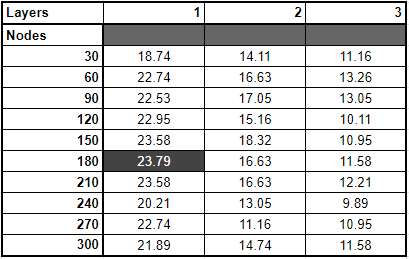
\includegraphics[scale=0.9]{images/Accuracy_table_lab_3.PNG}
    \caption{Accuracy Table}
    \label{fig:acc_table}
\end{figure}

\subsection{Results}
The accuracy table below shows clearly what the  number of nodes and layers were and what the accuracy was as shown in the table in Figure \ref{fig:acc_table}.

It can be observed that the accuracy of the network decreases with higher number of hidden layers. Within a certain number of layers, the accuracy does not vary too much.

Upon training the model with these parameters, a validation accuracy of 26.36\% was achieved. This model is selected assuming it to be the best model. The testing accuracy of this model is 26.67\%.

\section{Conclusion}
Even though the accuracy achieved is not at all satisfactory, the need and use of hyperparameter tuning, can be clearly seen. Hyperparameter tuning is a very essential and effective method in Deep Learning. It is useful in finding the optimal model and is one of the most important reason for Deep Learning to be relevant in the real world.

\end{document}
